
\subsubsection{Firms}

Finally with the industries defined, firms can be selected. 
To be able to find as much information as possible multinational \pharma companies have been selected from both the European and Indian markets.\\
The Indian \pharma companies are Ranbaxy and Cipla.\\ %(possibly Dr Reddy's).
The choice of these two companies is base on the size, they are among the largest in India and have a decent amount of growth (see Figure~\ref{fig:IndiaPharma}).

\begin{figure}[htbp] 
	\centering
	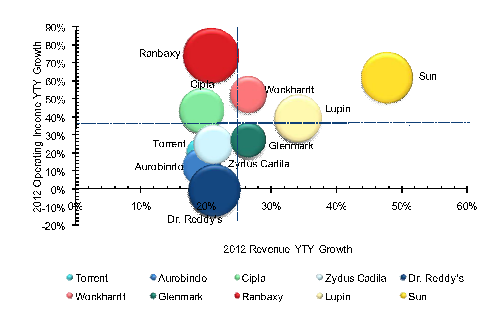
\includegraphics[width=0.8\textwidth]{IndiaPharma.eps}
 	\caption[Competitive Landscape of the Top 10 Pharmaceutical Companies in India]{Competitive Landscape of the Top 10 Pharmaceutical Companies in India, 2012. source:~\citep{Research-and-Markets:2013}}\label{fig:IndiaPharma}
\end{figure}

Many European \pharma companies have merged with or have been purchased by US firms. 
The focus will be on firms that have no original ties with the US through mergers.
This limitation has been considered to be able to include only firms into the research, that have the most European pedigree as possible.
As counterparts for the Indian firms we will choose Novartis and GSK as the European contenders.
Both the European firms are top 20 of \pharma~companies\footnote{\url{http://www.contractpharma.com/issues/2013-07/view_features/top-20-pharma-report-/}} in the world.\\
As for the ICT services firms in India there is a lot of choice. 
Here we opt for pure Indian companies not only have their operations in India, but the management and ownership are Indian as well.
For these reasons, Infosys and WiPro have been selected. 
%(TCS) is used as a backup company as they are not purely a ICT company.
Both companies are among the largest~\gls{IT} services firms in India feature in Gartner's Magic Quadrant for~\gls{IT} services firms~\cite{Gartner:2013a} and not a subsidiary from a larger company.
This would be the fact with TCS as this is part of the Tata group.
 
For the European Firms the choice is less broad. 
Pure European ICT firm are not as prevalent as Indian ICT services firms~\citep{Deloitte:2010}. 
This said Capgemini and T-systems as well as Atos are all very good examples of international ICT services firm. 
There are a number of local (national) ICT services for a good diversity of information these are not included.\\
The choice of Capgemini and T-systems is explained through their ranking among the largest companies in their industry in Europe.
T-systems and Capgemini have roots in different European countries~\citep{capgemini:2013aa,T-systems:2013} (France and Germany) this could provide an additional richness of data.\\
The firms in their respected economic areas and industries will be summarised in table~\ref{tab:firms}.

\begin{table}
  \centering
  \caption[Firms of under investigation]{Firms of under investigation. Source Author}\label{tab:firms}%
\begin{tabularx}{0.6\textwidth}{lXX} 
 % \toprule
 & \de (EU)& \ee (India)\\ 
  %\midrule 
  \midrule
  Services & Capgemini& Infosys \\
Industry  &T-Systems&WiPro\\
   \midrule
 Manufacturing &Novatis&Ranbaxy\\
 Industry &GSK & Cipla\\
  \bottomrule
  \end{tabularx}
\end{table}

The Firms will be described in more detail in the following section.

\paragraph{Detailed description of the firms}\label{sec:sevicesFirms}

The way~\gls{IT} services firms operates within the~\gls{IT} services business is largely similar for Indian or European firms~\cite{Gardner:2013}. 
Therefor these working practices are described for the entire sector and not repeated in table~\ref{tab:ServfirmsDescriptions}.
\gls{IT} services firms generally provide~\gls{IT} maintenance and development through outsourcing (in near or offshore locations) and~\gls{BPO} services~\citep{Wipro:2013aa,Infosys:2013aa,capgemini:2013aa,T-systems:2013}. 

The majority of \mne~have their own (proprietary)~\gls{IT} application landscape that is vital to their operations~\citep{Willcocks:2004ce}. 
As part of the application management services,~\gls{IT} services firms can maintain the current~\gls{IT} application landscape and also develop new applications (or replace applications build with old technology) that are specifically tailored for their clients~\citep{Cusumano:2008ta}.
The~\gls{IT} services firms typically, by acquiring the account to maintain and develop the~\gls{IT} applications, take over part of the personnel that was working at outsourcing company. 
Subsequently (a large) part of the development work done, is transferred to low-wage-countries~\citep{Barthelemy:2001ui}. 
The employees of these companies are located both in the home country of the client and in the home country of the~\gls{IT} services firms~\citep{Lacity:2009dk}.
The trend that has been observed is, these companies want to focus on their core business~\citep{Willcocks:2004ce}. 
As~\gls{IT} is not their core business they outsource this to other companies or set up a second company to perform these services~\citep{Earl:2012vd}. 
Firms that are more heavily~\gls{IT} reliant are telecommunications and financial services firms~\citep{Gonzalez:2006eh}. 
Some~\gls{IT} services firms started life as subsidiary that is operating (semi) independently, this is the case with T-Systems or have a spin-of company that is now competing in the market on its own~\citep{T-systems:2013}. 
Others started out as pure~\gls{IT} firms that have grown to become~\gls{IT} services firms partly by insourcing employees from their (former) customers~\citep{Barthelemy:2001ui}. 
The firms in the~\gls{IT} services area are described in table~\ref{tab:ServfirmsDescriptions}.

%\newpage
\begin{sidewaystable}
  %\tablefootnote{}
  \centering
  \caption[Services Firm Details]{Services Firm Details. Source Author}\label{tab:ServfirmsDescriptions}%
   \footnotesize
\begin{tabular}{lp{4cm}p{4cm}p{4cm}p{4cm}} 
 % \toprule

 \textbf{FirmName} 
& \includegraphics[width=.14\textwidth]{capgemini_logo.eps}      
& 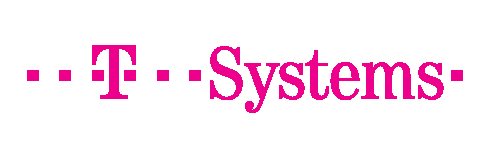
\includegraphics[width=.145\textwidth]{T-systems_logo.eps} 
& \includegraphics[width=.08\textwidth]{wipro_logo_BB.eps} 
& 
\includegraphics[width=.08\textwidth]{infosys_logo.eps}\\
 
 \textbf{Economy}             & \glsdesc{AE}           & \glsdesc{AE}   & \glsdesc{EE}  & \glsdesc{EE}\\
 
 \textbf{Industry Type}     & ICT Services     & ICT Services & ICT Services & ICT Services\\
  
 \textbf{Home Country}       & France         & Germany & India   & India\\
 
 \textbf{Employees}          & 100.000+       &  48.000 & 135.000 &150,000+\\
 
  \textbf{Year Founded}   & 1967   & 2000  & 1945 & 1981\\
 
 \textbf{2012 Revenue (in \euro)}     & \euro~10.26Bn     & \euro~10.02Bn 
 & \euro \pgfmathdivide{337.340}{\ExRupee} \pgfmathprintnumber[precision=2]{\pgfmathresult}Bn\tablefootnote{revenue was posted as \rupee~(337.340Bn) using table~\ref{tab:currencies} Euro value was calculated} 
 & \euro \pgfmathdivide{433.608}{\ExRupee} \pgfmathprintnumber[precision=2]{\pgfmathresult}Bn\tablefootnote{revenue was posted as \rupee~(433.608Bn) using table~\ref{tab:currencies} Euro value was calculated}\\
 
 \textbf{2012 Profit\tablefootnote{The Ebitda has been used to measure the profit of the companies} (in \euro)} &\euro~829Mn &\euro~350Mn 
 &
 \euro \pgfmathdivide{74.142}{\ExRupee} \pgfmathprintnumber[precision=2]{\pgfmathresult}Bn\tablefootnote{revenue was posted as \rupee~(74.142Bn) using table~\ref{tab:currencies} Euro value was calculated} 
 &
 \euro \pgfmathdivide{100.61}{\ExRupee} \pgfmathprintnumber[precision=2]{\pgfmathresult}Bn\tablefootnote{revenue was posted as \rupee~(100.61Bn) using table~\ref{tab:currencies} Euro value was calculated} \\
 
 \midrule
 \textbf{Description} &
  
Capgemini is a listed company at the Euronext stock exchange in Paris. The  main business of Capgemini are ICT and consulting services. The latter was acquired via a takeover of Ernst\& Young Consulting. \newline The name came to be from a merger between CAP, Sogeti and Gemini inc. Now Sogeti is wholly owned daughter of Capgemini. Typical clients are found in large manufacturing companies, banking and insurance, but also the public sector and healthcare.  &

 T-systems is a subsidiary of Deutsche Telekom AG\@. 
 Although a subsidiary it does serve other customers than DT\@. 
 The main activities are~\gls{IT} consulting and~\gls{IT} services. 
 These include minting the~\gls{IT} application landscape and building new applications specific for the client. 
 Typical clients are found in large manufacturing companies, banking and insurance, but also the public sector. &
 
WiPro is an Indian ICT services company, that unlike others started of as an company that manufactured oils, soaps and waxes as the `Western India Vegetable Products'.
 This heritage is still maintained in its company logo of a sunflower. 
In 1981 WiPro diversifies into~\gls{IT} services. The business is now known for. \newline 
Their main clients other \glspl{MNE}~that are located in the financial services, healthcare, manufacturing and telecommunications domains. &
In 1981 Infosys Consultants was established. In 1992 the name was changes to Infosys Technologies. Infosys is a NYSE listed global consulting and~\gls{IT} services company stemming from India. 
Similar to other Indian~\gls{IT} services firms the clients are \glspl{MNE}~that are located in the financial services, healthcare, manufacturing and telecommunications domains \\
  \bottomrule 
  \end{tabular}
\end{sidewaystable}



In general in the pharmaceutical business one can distinguish four phases in the process of the drug to hitting the market.
The drug has to be researched (a) and than (b) developed, then is has to be manufactured (c) and finally it has to be marketed and sold (d)~\citep{Paul:2010ff}. 
The research and development stages are among the most cash intensive processes in the \pharma industry.
To come up with a new (blockbuster) drug is extremely costly~\citep{Munos:2009bg} .
The drugs have to be approved by the appropriate authorities\footnote{These are the \gls{FDA} in the US and the \gls{EMA} in Europe}. 
Manufacturing and marketing of the drug can begin only after approval has been received~\citep{Kessel:2011go}.\\
Normally a drug that has been newly developed will also be granted a patent for a certain number of years. 
After the patent expires the drug can be \manu by anyone~\citep{Kaitin:2009dg}.
This dug becomes a so-called generic drug. 
Manufacturing generic drugs can have different implications compared to manufacturing proprietary drugs~\citep{Kessel:2011go}.

Indian \pharma companies have seen tremendous growth between 1970 and 1991~\citep{Chaturvedi:2006da,Bruche:2011uf}.
In 1970 the Patent Act was passed, which allowed the domestic manufacturing and marketing of patented products without a licence.
This fuelled a large reverse-engineering spree of patented drug by (almost all) Indian \pharma companies~\citep{Bruche:2011uf}.
This practice was halted in 1991 with the signing of~\gls{trips}. 
\gls{trips} marked the turning point of Indian policy regime towards the world~\citep{Chaturvedi:2006da}.
The reverse engineering practices came to a halt. 
The new patent regime that did not allow reverse engineering of known molecules, together with the pressure exerted by liberalisation and globalisation, is forcing firms to transform their R\&D activities and realign their competencies~\citep{Chaturvedi:2006da}.

%\newpage
\begin{sidewaystable}
  \centering
  \caption[Manufacturing Firm Details]{Manufacturing Firm Details. Source Author}\label{tab:ManfirmsDescriptions}
   \footnotesize
\begin{tabular}{lp{3cm}p{3cm}p{5.5cm}p{4.3cm}}  
 \textbf{Firm Name}           & 
\includegraphics[width=.12\textwidth]{novartis_logo.eps}    & 
\includegraphics[width=.12\textwidth]{gsk_logo.eps}   &  \includegraphics[width=.13\textwidth]{ranbaxy_logo2}    &\includegraphics[width=.09\textwidth]{Cipla_Logo.jpg}\\
 \toprule
 \textbf{Economy}             & \de          & \de   & \ee  & \ee\\
 
 \textbf{Industry Type}     &  \manu     & pharma \manu & pharma \manu & pharma \manu\\
  
 \textbf{Home Country}    & Switzerland             & UK & India& India\\
 
 \textbf{Employees}          & 120.000+       &  95.000 & 10.000+ &16,000+\\
 
 \textbf{Year Founded}    & pre 1900    &pre 1900  & 1961   & 1935 \\
 
 \textbf{2012 revenue (in \euro)}             
 &
 \euro~\pgfmathdivide{56.7}{\ExDollar} \pgfmathprintnumber[precision=2]{\pgfmathresult}Bn\tablefootnote{revenue was posted as \$~56.7Bn  using table~\ref{tab:currencies} Euro value was calculated}
   &
 \euro~\pgfmathdivide{26}{\ExPound} \pgfmathprintnumber[precision=2]{\pgfmathresult}Bn
\tablefootnote{revenue was posted as \pounds~26Bn  using table~\ref{tab:currencies} Euro value was calculated}
 &
 \euro \pgfmathdivide{123}{\ExRupee} \pgfmathprintnumber[precision=2]{\pgfmathresult}Bn
\tablefootnote{revenue was posted as \rupee 123Bn using table~\ref{tab:currencies} Euro value was calculated}
 &
 \euro \pgfmathdivide{85.24}{\ExRupee} \pgfmathprintnumber[precision=2]{\pgfmathresult}Bn
\tablefootnote{revenue was posted as \rupee 85.24Bn using table~\ref{tab:currencies} Euro value was calculated} 
 \\
 %total operating profit
\textbf{2012 Profit\tablefootnote{The Ebitda has been used to measure the profit of the companies} (in \euro)}   &\euro~\pgfmathdivide{11.511}{\ExDollar} \pgfmathprintnumber[precision=2]{\pgfmathresult}Bn  
& 
\euro~\pgfmathdivide{7.4}{\ExPound} \pgfmathprintnumber[precision=2]{\pgfmathresult}Bn
&
 \euro \pgfmathdivide{-1642.83}{\ExRupee} \pgfmathprintnumber[precision=2]{\pgfmathresult}Mn
  &
  \euro \pgfmathdivide{122.4}{\ExRupee} \pgfmathprintnumber[precision=2]{\pgfmathresult}Bn\\
 \midrule
 \textbf{Description} &
  
Novartis is the product of a merger between Ciba-Geigy and Sandoz Laboratories in 1996. In this merger the \pharma devisions continued operation under the name Novartis while the other operations were divested. Novartis engages in research, development, manufacturing and marketing of prescription (proprietary) drugs. These four stages mentioned earlier.
\cite{businessweek:Novartis}

&
GlaxoSmithKline in full or GSK, was formed through a merger of Glaxo Wellcome and SmithKline Beecham in 2000. GSK has a portfolio of products for major diseases and also a large consumer healthcare division. GSK engages  research, development, manufacturing and marketing of prescription and over-the-counter drugs.
\cite{Businessweek:GSK}
&
Ranbaxy was founded in 1937 as a distributor of Japanese manufactured drugs. 
The name Ranbaxy is a aggregation of the names of its first owners \textbf{Ran}bir and Gur\textbf{bax}.   
In 2008 Daiichi Sankyo of Japan acquired a controlling share in Ranbaxy.
Ranbaxy however remains listed on the Indian stock exchange. 
\newline
In later stages Ranbaxy developed~\gls{ndds} techniques, thereby adding their own value to the existing products.
There is an tendency though seen at Ranbaxy to seriously pursue new drug discovery programmes. It is suggested that Ranbaxy, generally,  has been investing more in the R content of R\&D and have gradually moved away from reverse engineering~\cite{Chaturvedi:2006da}.
However the bulk of the Ranbaxy business lies in manufacturing, marketing (and selling) pharmaceuticals products\cite{Businessweek:Ranbaxy,maheshsundar:2013}
&
Cipla was founded as the Chemical, Industrial and Pharmaceutical Laboratories in 1935. 
Nowadays it is better known as its acronym then by its full name.
 Cipla \manu OTC prescriptions drugs. 
 Next to this they also manufacture \gls{API} and drug intermediates. 
 \newline 
Cipla is engaged in manufacture and marketing (sales) of pharmaceutical products in India and internationally.
Cipla focusses on improving their manufacturing efficiency and establishing large production facilities. Cipla has invested more in the D content and have strengthened their infrastructure and financial position through process efficiencies, economies of scale and large product baskets rather than research\cite{Chaturvedi:2006da}.\\
  \bottomrule 
  \end{tabular}
\end{sidewaystable}